\section{American Option Pricing}

\subsection{Options}

\begin{remark}
    \vocab{Options} are financial instruments whose payoff depends on an \vocab{underlying asset}. More generally, they are \vocab{contingent claims}.
\end{remark}

\begin{definition}
    Consider a financial market with vector price process $S$. A \vocab{contingent claim} with maturity $T$ is any stochastic variable $\mc{X} \in \mc{F}_T^S$. It is called \vocab{simple} if $\mc{X} = g(S(T))$.
    
    The function $g$ is the \vocab{contract function}. At time $T$ we will know the payoff.
\end{definition}

\begin{itemize}
    \item \vocab{European options}: These are examples of simple contingent claims, with contract functions:
    \begin{itemize}
        \item \vocab{Call option}: $g(x) = \max[x-K, 0] = (x-K)^+$
        \item \vocab{Put option}: $g(x) = \max[K-x, 0] = (K-x)^+$
    \end{itemize}
    
    \item \vocab{American options}: The option can be exercised prior to time $T$. The choice of the time of exercise is left to the holder of the option.
\end{itemize}

\begin{remark}
    At time $t$, if the option is exercised, the payoff is $g(S_t)$. The decision to exercise at time $t$ can be made based on the information available up to that time, $\mc{F}_t^S$. From the point of view of $t=0$, the exercise time will be a random variable $\tau$, which will be a \vocab{stopping time}.
    
    The central problem with options is to determine the \vocab{fair price} of the claim $\pi(t, g)$ for $t \leq T$.
    
    If $t=T$, we know $\pi(T, g) = g(S(T))$ for a simple claim. But what if $t < T$?
    
    Let us review pricing of contingent claims, taking a discrete-time approach first, which naturally evokes the use of \vocab{backward induction} methods.
    
    In the first part of the course, you learned how to address:
    \[ V_* = \sup_\tau \EE[G_\tau]. \]
    How is this connected to American options pricing?
\end{remark}

\subsubsection{Preliminaries: 1-period model}

\begin{remark}
    Key concepts: $\PP$ measure, replicating portfolios, martingale measure, arbitrage pricing.
    
    Consider the simplest set-up: a \vocab{1-period model}.
    \begin{itemize}
        \item $S_0$: current price of a stock.
        \item $K$: strike price.
        \item $T = 1$ period.
        \item $r$: risk-free interest rate.
        \item $\Omega = \{\omega_1, \omega_2\}$.
    \end{itemize}
    The stock price at maturity is:
    \[ S_T(\omega) = \begin{cases} S^u & \omega = \omega_1 \\ S^d & \omega = \omega_2 \end{cases} \]
    The payoff of a call option at maturity is $C_T = (S_T - K)^+$. Specifically:
    \[ C_T(\omega) = \begin{cases} S^u - K & \omega = \omega_1 \\ 0 & \omega = \omega_2 \end{cases} \]
    (assuming $S^u > K$ and $S^d < K$).
    
    What is the fair price $C_0$? It is rational to define a "fair" price as the \vocab{expected discounted (present) value} of the terminal payoff of the option:
    \[ \EE \left[ (1+r)^{-1} C_T \right]. \]
    This requires an evaluation of the probability that $\omega = \omega_1$ and $\omega = \omega_2$. This leads to the \vocab{choice of the measure}!
\end{remark}

\begin{remark}
    One possible (natural) choice for pricing is to use the measure that reflects the investor's assessment of probabilities: the \vocab{subjective probability} $\PP$ measure (actual, real-world).
    However, different investors have different views, which would lead to different prices $C_0$. We need a different measure, in a model that guarantees a unique price.
\end{remark}

\begin{remark}[Replicating Portfolio]
    The idea is to construct a \vocab{synthetic portfolio} (a mix of securities) such that it replicates the payoff of the contingent claim at time $T$.
    Consider two assets:
    \begin{itemize}
        \item The stock on which the option is written.
        \item A bank account.
    \end{itemize}
    Let $\phi_0 = (\alpha_0, \beta_0)$ be the portfolio at time $0$, and $V_t(\phi)$ be the value of the portfolio at time $t$.
    Then:
    \[ V_0(\phi) = \alpha_0 S_0 + \beta_0, \quad V_T(\phi) = \alpha_0 S_T + (1+r) \beta_0. \]
    We say $\phi$ is a \vocab{replicating portfolio} for $C$ if $V_T(\phi) = C_T$. In our 2-state model, this means:
    \[ V_T(\phi) = \begin{cases} V^u(\phi) = \alpha_0 S^u + (1+r) \beta_0 = C^u & \text{if } \omega = \omega_1 \\ V^d(\phi) = \alpha_0 S^d + (1+r) \beta_0 = C^d & \text{if } \omega = \omega_2 \end{cases} \]
    In this setup, it is possible to find the portfolio $(\alpha_0, \beta_0)$ constructed at time $0$ s.t. the payoff of the option is replicated. Then, the cost of the contingent claim can be defined as the investment needed to construct the replicating portfolio:
    \[ C_0 = V_0(\phi) = \alpha_0 S_0 + \beta_0. \]
    Notice that this price depends only on $S_0$ and is independent of the subjective probabilities of who prices!
\end{remark}

\begin{remark}[No Arbitrage Pricing]
    Given the replicating portfolio, we consider the following strategy:
    \begin{itemize}
        \item At $t=0$:
        \begin{itemize}
            \item sell the contingent claim: $+C_0$
            \item buy $\alpha_0$ stocks: $-\alpha_0 S_0$
            \item lend an amount $\beta_0$: $-\beta_0$
        \end{itemize}
        \item At $t=T$:
        \begin{itemize}
            \item payoff of the contingent claim: $-C_T$
            \item sell the stocks: $+\alpha_0 S_T$
            \item receive the loan back: $\beta_0(1+r)$
        \end{itemize}
    \end{itemize}
    We know that $\alpha_0 S_T + \beta_0(1+r)$ is always equal to $C_T$. If $C_0 \neq \alpha_0 S_0 + \beta_0$, then it would be possible to construct an \vocab{arbitrage}, i.e., a strategy that yields a sure profit at time $t=0$.
    If the model is \vocab{arbitrage-free}, then $C_0$ can be considered as the fair price of the claim.
\end{remark}

\begin{remark}[Martingale Measure]
    It is convenient to try to obtain the value of a contingent claim as the \vocab{expected discounted present value} of its cash flows:
    \[ C_0 = \EE \left[ (1+r)^{-1} C_T \right] \quad \text{under which measure?} \]
    The idea is to find a probability measure $\PP^*$ equivalent to $\PP$ s.t. the discounted price process is a \vocab{martingale}.
    For the stock, let $S_0^* = S_0$ and $S_T^* = (1+r)^{-1} S_T$. The martingale property requires:
    \[ S_0 = S_0^* = \EE_{\PP^*}[S_T^*] = \EE_{\PP^*}[(1+r)^{-1} S_T]. \]
    In our 2-state model, this is:
    \[ S_0 = (1+r)^{-1} [S^u p^* + S^d (1-p^*)], \quad \text{where } p^* = \PP^*\{\omega = \omega_1\}. \]
    Solving this equation for $p^*$:
    \[ S_0(1+r) = S^u p^* + S^d - S^d p^* \implies p^* = \frac{S_0(1+r) - S^d}{S^u - S^d}. \]
    Now we ask: is $C_0^* = \EE_{\PP^*}[(1+r)^{-1} C_T] = C_0$?
    From the replicating portfolio equations, we can find:
    \[ \alpha_0 = \frac{C^u - C^d}{S^u - S^d}, \quad \beta_0 = \frac{C^d S^u - C^u S^d}{(S^u - S^d)(1+r)}. \]
    Then:
    \begin{align*}
        C_0^* &= (1+r)^{-1} [C^u p^* + C^d (1-p^*)] \\
        &= (1+r)^{-1} \left[ C^u \frac{S_0(1+r) - S^d}{S^u - S^d} + C^d \paren{1 - \frac{S_0(1+r) - S^d}{S^u - S^d}} \right] \\
        &= (1+r)^{-1} \left[ \frac{S_0(1+r)}{S^u - S^d} (C^u - C^d) + \frac{C^d S^u - C^u S^d}{S^u - S^d} \right] \\
        &= S_0 \frac{C^u - C^d}{S^u - S^d} + (1+r)^{-1} \frac{C^d S^u - C^u S^d}{S^u - S^d} \\
        &= S_0 \alpha_0 + \beta_0 = C_0.
    \end{align*}
    We have now established the link between $C_0$ and $C_0^*$. However, in order to exclude arbitrage, we need to further assume that $C_0$ is always non-negative.
\end{remark}

This transcription follows the style and structure of your provided preamble and previous chapter, using the defined environments and commands.

\section{Arbitrage-Free Pricing and American Options}

\begin{definition}
    A pricing model $M$ is \vocab{arbitrage-free} if there exists no portfolio $\Phi$ such that:
    \[ V_0(\Phi) = 0, \quad V_T(\Phi) \geq 0, \quad \mathbb{P}[V_T(\Phi) > 0] > 0 \]
    or if there is no portfolio such that:
    \[ V_0(\Phi) < 0, \quad V_T(\Phi) \geq 0 \implies \text{\vocab{Strong Arbitrage}} \]
    If the market is arbitrage-free, then $C_0^*$ is the \vocab{no-arbitrage price}.
\end{definition}

\begin{proposition}
    To conclude this recap, consider $S_T = \begin{cases} S^u & \omega = \omega_1 \\ S^d & \omega = \omega_2 \end{cases}$ and $B_0 = 1, B_T = 1+r$. Let $\Phi$ be the linear space of portfolios of $S$ and $B$.
    
    The market $M = (S, B, \Phi)$ is arbitrage-free if and only if $S^*$ admits a \vocab{martingale measure} $\mathbb{P}^*$. Then, the arbitrage-price of any contingent claim $C_T$ that settles at $T$ is given by:
    \[ C_0 = \mathbb{E}_{\mathbb{P}^*} \left[ (1+r)^{-1} C_T \right] \]
\end{proposition}

\begin{remark}
    Let us now consider \vocab{American options} in this setup. Since there are only 2 dates, the option can be exercised either at $0$ or at $1$.
    
    How to price an American claim? We want to find $\pi_0(X^a)$.
    \begin{itemize}
        \item \textbf{At maturity:} $X_1^a = X_T \implies$ equivalent to a European claim.
        \item \textbf{At time 0:} The holder has the option to exercise. The decision is optimally (rationally) taken by comparing the immediate payoff to the expected payoff obtained at maturity.
    \end{itemize}
\end{remark}

\begin{proposition}
    \textbf{Price of an American Call.} Assume $S^d < K < S^u$. Assume $r \geq 0$ and $S^d < S_0(1+r) < S^u$. Then $C_0^a = C_0^e$.
\end{proposition}

\begin{proof}
    Assume the contrary, i.e., $C_0^a > C_0$ at first. First, notice that:
    \begin{align*}
        C_0 &= \mathbb{E}^* \left[ (1+r)^{-1} (S_T - K)^+ \right] \\
        &= (1+r)^{-1} p^* [S^u - K] \\
        &= \frac{(1+r)S_0 - S^d}{S^u - S^d} \cdot \frac{S^u - K}{(1+r)}
    \end{align*}
    Notice that:
    \[ \frac{(1+r)S_0 - S^d}{S^u - S^d} \cdot \frac{S^u - K}{(1+r)} = \left( S_0 - \frac{S^d}{1+r} \right) \cdot \frac{S^u - K}{S^u - S^d} \]
    Since $K > S^d$, we have $S^u - K < S^u - S^d$, which implies $\frac{S^u - K}{S^u - S^d} < 1$. However, we also observe:
    \[ S_0 - \frac{S^d}{1+r} > S_0 - K \quad \text{since } K > S^d \text{ and } r \geq 0 \]
    This leads to the conclusion that $C_0 > S_0 - K$.
    
    Therefore, if $C_0^a > C_0$, we can sell the American call option at $C_0^a$ and buy the European call option at $C_0$.
\end{proof}

\begin{remark}
    The arbitrage strategy can be summarized by the following payoff table:
    
    \begin{center}
    \begin{tabular}{|l|c|c|c|}
    \hline
    \textbf{Action} & \textbf{Time 0} & \textbf{If ex. at 0} & \textbf{Time 1 (if not ex.)} \\ \hline
    Sell American & $+C_0^a$ & $-(S_0 - K)$ & $-(S_T - K)^+$ \\ \hline
    Buy European & $-C_0$ & $0$ & $(S_T - K)^+$ \\ \hline
    \textbf{Net} & $C_0^a - C_0 > 0$ & $C_0^a - (S_0 - K)$ & matched \\ \hline
    \end{tabular}
    \end{center}

    \begin{itemize}
        \item \textbf{At 0 if exercised:} The profit is $C_0^a - (S_0 - K)$. Since $C_0^a \geq C_0$ and we showed $C_0 > S_0 - K$, this is strictly positive.
        \item \textbf{If not exercised:} We buy $C_0$ and put $C_0^a - C_0 > 0$ in the bank at time 0. At time 1, the payoffs are matched, leaving the initial profit.
    \end{itemize}
\end{remark}

\begin{homework}
    Describe the arbitrage when $C_0^a < C_0$.
\end{homework}

This transcription follows the style and structure of your provided preamble and previous chapter, using the defined environments and commands.

\section{American Put Pricing}

\begin{proposition}
    \textbf{American Put Price.} Assume $r > 0$, $S^d < S_0(1+r) < S^u$, and $S^d < K < S^u$. Then, $P_0^a = P_0$ if and only if
    \begin{equation}
        K - S_0 \leq \frac{S^u - (1+r)S_0}{S^u - S^d} \cdot \frac{K - S^d}{1+r} \tag{$*$}
    \end{equation}
    Otherwise, $P_0^a = K - S_0 > P_0$. If $r = 0$, then $P_0^a = P_0$.
\end{proposition}

\begin{proof}
    Notice that
    \begin{align*}
        P_0 &= \EE^* \left[ (1+r)^{-1} (K - S_T)^+ \right] \\
        &= \frac{1}{1+r} (1 - p^*) (K - S^d) \\
        &= \frac{K - S^d}{1+r} \cdot \frac{S^u - (1+r)S_0}{S^u - S^d}
    \end{align*}
    and indeed $(*)$ is equivalent to $P_0 \geq K - S_0$.

    Suppose first the inequality holds. If $P_0^a > P_0$, one can create an arbitrage by selling the American put and buying the European put.
    
    \begin{homework}
        Write the payoffs of the strategy described above.
    \end{homework}
    
    Hence, $P_0 = P_0^a$. Now suppose $(*)$ does not hold, which implies $P_0 < K - S_0$.
    
    Assume $P_0^a \neq K - S_0$. We want to prove by contradiction that, if this is the case, arbitrage opportunities exist.
    \begin{itemize}
        \item If $P_0^a > K - S_0$, we can sell the American put and buy the European put at a lower price since $P_0 < K - S_0$.
        \item If $P_0^a < K - S_0$, we can buy the American put and exercise it immediately, yielding a profit of $(K - S_0) - P_0^a > 0$. This implies $P_0^a = K - S_0$, which is a contradiction.
    \end{itemize}
    Also, if $P_0 < K - S_0$, it must be that $P_0^a = K - S_0 > P_0$.
    
    If the holder of the put fails to exercise it at time 0, the option writer is still able to lock in a profit. Thus, if $P_0 < K - S_0$, either $P_0^a$ is exercised immediately or arbitrage opportunities arise.
    
    If $r = 0$, the condition $K - S_0 \leq \frac{S^u - S_0}{S^u - S^d} (K - S^d)$ is always valid.
\end{proof}

\begin{remark}
    Notice that the relation $C_0 = C_0^a$ is more general. Consider $S_T$ to be a $\PP^*$-integrable random variable. Then if $r \geq 0$, we have by \vocab{Jensen's inequality}:
    \begin{align*}
        \EE_{\PP^*} \left[ (1+r)^{-1} (S_T - K)^+ \right] &\geq \left( \EE_{\PP^*} \left[ (1+r)^{-1} S_T - (1+r)^{-1} K \right] \right)^+ \\
        &= \left( S_0 - (1+r)^{-1} K \right)^+ \geq S_0 - K
    \end{align*}
    and then $C_0 = C_0^a$ even in this setup.
    
    For the put option, we have:
    \begin{align*}
        \EE_{\PP^*} \left[ (1+r)^{-1} (K - S_T)^+ \right] &\geq \left( \EE_{\PP^*} \left[ (1+r)^{-1} K - (1+r)^{-1} S_T \right] \right)^+ \\
        &= \left[ (1+r)^{-1} K - S_0 \right]^+
    \end{align*}
    Note that $\left[ (1+r)^{-1} K - S_0 \right]^+ > K - S_0$ if $-1 < r < 0$.
    
    If $r = 0$, then the lower bound is $K - S_0$.
    
    If $r > 0$, no obvious relationship between $P_0$ and $S_0 - K$ exists.
\end{remark}

\begin{remark}
    Let us now focus on the \vocab{"rational" exercise rule} (which extends to the case of a discrete multi-period setup or to a continuous time setup).
    
    At any $t$ before expiration, it is necessary to find the maximal possible expected payoff over all admissible exercise rules (under the \vocab{risk-neutral measure}!) and compare it to the payoff received by exercising immediately.
    
    \textbf{Assumption:} exercise is executed at the dates for which subjective probabilities = risk-neutral ones.
\end{remark}

\begin{proposition}
    The arbitrage prices of an American call and an American put in an arbitrage-free market with $t = \{0, 1\}$ are:
    \begin{align*}
        C_0^a &= \max_{\tau \in \mc{T}} \EE_{\PP^*} \left[ (1+r)^{-\tau} (S_\tau - K)^+ \right] = \max \paren{ (S_0 - K)^+, \EE_{\PP^*} \left[ (1+r)^{-1} (S_1 - K)^+ \right] } \\
        P_0^a &= \max_{\tau \in \mc{T}} \EE_{\PP^*} \left[ (1+r)^{-\tau} (K - S_\tau)^+ \right] = \max \paren{ (K - S_0)^+, \EE_{\PP^*} \left[ (1+r)^{-1} (K - S_1)^+ \right] }
    \end{align*}
    where $\mc{T}$ is the set of exercise times, $\mc{T} = \{0, 1\}$.
    
    In general, if $X^a = (X_0, X_T)$ is an American contingent claim, its arbitrage price $\pi(X^a)$ is:
    \[ \pi(X^a) = \max_{\tau \in \mc{T}} \EE_{\PP^*} \left[ (1+r)^{-\tau} X_\tau \right] \]
    where $\pi(X_T^a) = X_T$ (cf. problem of Ch. 3, 1st part of the course!).
\end{proposition}

\section{Binomial Pricing}

\begin{remark}
    Let us consider a discrete-time setup to see the \vocab{backward induction} method at play and learn about a methodology to price contingent claims, \vocab{Binomial Pricing} (Cox, Ross, Rubinstein 1979).
    
    \begin{itemize}
        \item \textbf{Dates:} $0, 1, \dots, T^*$
        \item \textbf{Assets:} 
        \begin{itemize}
            \item $S \to$ stock: $\xi_{t+1} = \frac{S_{t+1}}{S_t} \in \{u, d\} \ \forall t, \ 0 < d < u$. \\
            $S_0 > 0$; $\PP(S_{t+1} = u S_t | \mc{F}_t) > 0$; $\PP(S_{t+1} = d S_t | \mc{F}_t) > 0$.
            \item $B \to$ bank account: $B_0 = 1, B_t = (1+r)^t$.
        \end{itemize}
    \end{itemize}
    Assume $\PP(\xi_t = u) = p = 1 - \PP(\xi_t = d), \ \forall t$. For no arbitrage, we require $0 < d < 1+r < u$.
    
    The stock price at time $t$ is $S_t = S_0 \prod_{j=1}^t \xi_j$. Let $\mu_j = \log \xi_j$ be the \vocab{log-returns}, which are i.i.d.
\end{remark}

\begin{remark}
    We now focus on contingent claim pricing in this model. Let us consider a simple claim first, with maturity $T \leq T^*$, $X = g(S_T)$ (path independent).
    
    To determine the arbitrage price of $X$ at any $t \in \mc{T}$, we show that it is possible, at any $t$, to consider a portfolio $\phi_t = (\alpha_t, \beta_t)$ of positions in $S$ and $B$ that replicates the payoff of $X$ at time $T$.
    
    The portfolio $\phi_t$ is a \vocab{dynamic, replicating, self-financing portfolio (strategy)}.
    
    Backward induction can be readily used, since $X_T$ is known. We start by considering $[T-1, T]$ and constructing the replicating portfolio at $T-1$. $\phi_{T-1} = (\alpha_{T-1}, \beta_{T-1})$ must be s.t.
    \[ V_T(\phi) = \alpha_{T-1} S_T + \beta_{T-1} (1+r) \]
    replicates the payoff of $X_T = g(S_T) = \begin{cases} g(S_{T-1} \cdot u) & \text{if } \xi_T = u \\ g(S_{T-1} \cdot d) & \text{if } \xi_T = d \end{cases}$
    
    Hence:
    \[ \begin{cases} \alpha_{T-1} u S_{T-1} + \beta_{T-1} (1+r) = g(S_{T-1} \cdot u) \\ \alpha_{T-1} d S_{T-1} + \beta_{T-1} (1+r) = g(S_{T-1} \cdot d) \end{cases} \]
\end{remark}

\begin{homework}
    Show that solving the system above yields:
    \[ \alpha_{T-1} = \frac{g(S_{T-1} u) - g(S_{T-1} d)}{u S_{T-1} - d S_{T-1}} \]
    \[ \beta_{T-1} = (1+r)^{-1} \frac{g(S_{T-1} d) u S_{T-1} - g(S_{T-1} u) d S_{T-1}}{u S_{T-1} - d S_{T-1}} \]
    Note that $\alpha_{T-1}, \beta_{T-1}$ are functions of $S_{T-1}$.
    
    Also, show that the value of the portfolio at $T-1$ is:
    \[ V_{T-1}(\phi) = \alpha_{T-1} S_{T-1} + \beta_{T-1} = (1+r)^{-1} \left[ p^* g(S_{T-1} u) + (1 - p^*) g(S_{T-1} d) \right] \]
    where $p^* = \frac{(1+r) - d}{u - d}$ is the \vocab{risk-neutral probability}. Note that $p^* \in (0, 1)$ requires $d < 1+r < u$.
\end{homework}

\begin{remark}
    Assuming absence of arbitrage (and following the reasoning of the 1-period model), $V_{T-1}(\phi)$ is the value of the contingent claim $X$ at time $T-1$:
    \[ X_{T-1} = V_{T-1}(\phi) \]
    This is a function of $S_{T-1}$!
\end{remark}

\begin{remark}
    We can now continue backwards, consider $[T-2, T-1]$ and look for a portfolio $\phi_{T-2} = (\alpha_{T-2}, \beta_{T-2})$ that replicates $X_{T-1}$, i.e. s.t.
    \[ \alpha_{T-2} S_{T-1} + \beta_{T-2} (1+r) = X_{T-1} \]
    (notice that $\alpha_{T-2} S_{T-1} + \beta_{T-2} (1+r) = \alpha_{T-1} S_{T-1} + \beta_{T-1}$)
    \begin{center}
        (\vocab{self-financing})
    \end{center}
    
    Then:
    \[ \begin{cases} \alpha_{T-2} u S_{T-2} + \beta_{T-2} (1+r) = X_{T-1}^u \\ \alpha_{T-2} d S_{T-2} + \beta_{T-2} (1+r) = X_{T-1}^d \end{cases} \]
    where 
    \begin{align*}
        X_{T-1}^u &= (1+r)^{-1} \left[ p^* g(u \cdot S_{T-2} \cdot u) + (1-p^*) g(u \cdot S_{T-2} \cdot d) \right] \\
        X_{T-1}^d &= (1+r)^{-1} \left[ p^* g(d \cdot S_{T-2} \cdot u) + (1-p^*) g(d \cdot S_{T-2} \cdot d) \right]
    \end{align*}
    
    and, finding $\alpha_{T-2}, \beta_{T-2}$,
    \[ V_{T-2}(\phi) = \alpha_{T-2} S_{T-2} + \beta_{T-2} = (1+r)^{-1} \paren{ p^* X_{T-1}^u + (1-p^*) X_{T-1}^d } \]
    which, using the usual NA arguments, gives
    \[ X_{T-2} = V_{T-2}(\phi). \]
\end{remark}

\begin{remark}
    \vocab{Path-dependent claims}
    
    The feature of a path-dependent European claim is that its final payoff is $g(S_0, \dots, S_T)$. Consider a sample path $(s_0, s_1, \dots, s_{T-1})$. Consider the interval $[T-1, T]$. Then to find the replicating portfolio:
    \[ \begin{cases} \alpha_{T-1}(s_0, s_1, \dots, s_{T-1}) u S_{T-1} + \beta_{T-1}(s_0, \dots, s_{T-1})(1+r) = g^u \\ \alpha_{T-1}(s_0, s_1, \dots, s_{T-1}) d S_{T-1} + \beta_{T-1}(s_0, \dots, s_{T-1})(1+r) = g^d \end{cases} \]
    Note that $s_0$ and $S_{T-1}$ are connected by a number of paths.
    
    Thus, the price at $T-1$ is $\pi_{T-1}(X) = V_{T-1}(\phi) = \alpha_{T-1}(s_0, s_1, \dots, s_{T-1}) S_{T-1} + \beta_{T-1}(s_0, \dots, s_{T-1})$, which will be different at any node for each sample path connecting $s_0$ and $S_{T-1}$.
    
    As long as $\pi_{T-1}(X)$ can be found at $S_{T-1}$ for every possible path, we can apply the same procedure to obtain $\pi_{T-2}(X)$ by looking at $[T-2, T-1], \dots$, yielding a unique solution!
\end{remark}

\begin{remark}
    The binomial (CRR) model is \vocab{COMPLETE} because any European (path-dependent or independent) claim can be replicated; $V(\phi)$ and $\phi$ are adapted to the filtration generated by $S$, and $\pi(X) = V(\phi)$.
    
    The CRR model gives a closed-form formula for the price of a European call or put option (see MR p. 43--46 for the formula and proof).
\end{remark}

\section{No Arbitrage in the CRR model}

\begin{proposition}
    A martingale measure $\PP^*$ for $S^*$ exists iff $d < 1+r < u$. In this case, $\PP^*$ is the unique element of the class of probability measures such that $p^* = \frac{1+r-d}{u-d}$ and $S_t^* = \frac{S_t}{B_t} = S_t(1+r)^{-t}$.
\end{proposition}

\begin{proof}
    We want to show $\EE_{\PP^*}(S_{t+1}^* | \mc{F}_t^S) = S_t^*$.
    
    Since $S_{t+1} = \xi_{t+1} S_t$ for all $t < T^*$, we have:
    \begin{align*}
        \EE_{\PP^*}(S_{t+1}^* | \mc{F}_t^S) &= \EE_{\PP^*} \left[ S_t \xi_{t+1} (1+r)^{-(t+1)} \middle| \mc{F}_t^S \right] \\
        &= S_t (1+r)^{-(t+1)} \EE_{\PP^*} \left[ \xi_{t+1} \middle| \mc{F}_t^S \right]
    \end{align*}
    The condition $\EE_{\PP^*}(S_{t+1}^* | \mc{F}_t^S) = S_t^*$ implies:
    \[ (1+r)^{-(t+1)} S_t \EE_{\PP^*} \left[ \xi_{t+1} \middle| \mc{F}_t^S \right] = (1+r)^{-t} S_t \]
    Since $S_t > 0$, the equality holds iff:
    \[ \EE_{\PP^*}[\xi_{t+1} | \mc{F}_t^S] = 1+r \implies \EE_{\PP^*}[\xi_{t+1} | \mc{F}_t^S] = \EE_{\PP^*}(\xi_{t+1}) \]
    since $(1+r)$ is constant. This means $\xi_{t+1}$ is independent of $\mc{F}_t^S$ under $\PP^*$ and thus independent of $\xi_1, \dots, \xi_t$ for all $t$.
    
    Hence:
    \[ \EE_{\PP^*}[\xi_t] = u \PP^*\{\xi_t = u\} + d \PP^*\{\xi_t = d\} = 1+r \]
    Using $\PP^*\{\xi_t = d\} = 1 - \PP^*\{\xi_t = u\}$, we get:
    \[ u p^* + d(1-p^*) = 1+r \implies p^* = \frac{1+r-d}{u-d} \quad \forall t \]
\end{proof}

\begin{remark}
    From this result, it is clear that $\PP^*$ is a probability measure only if $d \leq 1+r \leq u$ and is equivalent to $\PP$ only if $d < 1+r < u$.
\end{remark}

\begin{homework}
    Why is $\PP^*$ equivalent to $\PP$ only if $d < 1+r < u$?
\end{homework}

\begin{remark}
    Hence, we have established that we can use the binomial model as an arbitrage pricing model!
    
    $p^*$ defines the martingale measure, with our choice of the \vocab{NUMERAIRE} $B_t$.
    
    Indeed:
\end{remark}

\begin{proposition}
    Consider a European call option. Then the arbitrage price formula obtained by evaluating by backward induction the replicating portfolios coincides $\forall m=0,1, \dots, T$ with
    \[ C_{T-m}^* = \EE_{\PP^*} \paren{ (1+r)^{-m} (S_T - K)^+ \mid \mc{F}_{T-m}^S } \]
\end{proposition}

\begin{proof}
    See Musiela and Rutkowski p. 50.
\end{proof}

\begin{remark}
    $\to$ Notice that the B-S pricing formula can be obtained as a limit version of the CRR formula.
\end{remark}

\section{American Options in the CRR Model}

\begin{remark}
    Recall that, given our "rational" reasoning about the exercise of the option; at any valuation time the holder prices the option as the max of the exercise value and the max (R-N) expected payoff that can be earned by exercising at any future possible exercise date.
    
    Reasoning by backward induction again:
    
    At $T$, we have $\pi_T(X_T) = X_T$.
    
    Consider $[T-1, T]$. Then, at $T-1$ the holder of the option can exercise immediately, obtaining $X_{T-1}$, or keep the option, valued $\EE_{\PP^*} \left[ (1+r)^{-1} X_T \mid \mc{F}_{T-1} \right] \implies$
    \[ \pi_{T-1} = \max \paren{ X_{T-1}, \EE_{\PP^*} \left[ (1+r)^{-1} X_T \mid \mc{F}_{T-1} \right] }. \]
    
    By induction, for every $t=1, \dots, T$
    \[ \pi_{t-1} = \max \paren{ X_{t-1}, \EE_{\PP^*} \left[ (1+r)^{-1} \pi_t \mid \mc{F}_{t-1} \right] }. \]
    (This is the \vocab{Snell envelope} $S_n(\omega)$ from ch. 3 - part 1!)
    
    And, as already said, $\pi_T = X_T$.
\end{remark}

\begin{remark}
    We know from the 1st part of the course that $(\tilde{\pi}_t)_{0 \leq t \leq T}$, where $\tilde{\pi}_t = (1+r)^{-t} \pi_t$ is the smallest supermartingale which dominates $(X_t)_{0 \leq t \leq T}$ and that $(\pi_t)_{0 \leq t \leq T}$ is the \vocab{Snell's envelope} of $(X_t)_{0 \leq t \leq T}$.
    
    We know also that $\tau_m^T$ s.t. $\pi_m = \EE \left[ X_{\tau_m^T} \mid \mc{F}_m \right]$ is the optimal stopping time.
    
    $\to$ Results extend to the case of $T \to +\infty$.
\end{remark}

%%%%%%%%%%%%%%%%%%%%%%%%%%%%%%%%%%%%%%%%%%%%%%%%%%%%%%%%%%%%%%%%%%%%%

\section{Call Option Pricing}

\begin{remark}
    As already hinted at, the case of a call option is peculiar. We first notice that denoting with $C_t$ the price of a call, the following inequality holds:
    \[ C_t \geq (S_t - K)^+ \quad \forall t \leq T \]
    Indeed, by \vocab{Jensen's inequality}:
    \begin{align*}
        \EE_{\PP^*} \left[ (1+r)^{-(T-t)} (S_T - K)^+ \mid \mc{F}_t^S \right] &\geq \paren{ \EE_{\PP^*} \left[ (1+r)^{-(T-t)} S_T - (1+r)^{-(T-t)} K \mid \mc{F}_t^S \right] }^+ \\
        &\geq (S_t - K)^+ \quad \forall t \leq T
    \end{align*}
    where we used the fact that $\EE_{\PP^*} \left[ (1+r)^{-(T-t)} S_T \mid \mc{F}_t^S \right] = S_t$ and $(1+r)^{-(T-t)} K \leq K$ (with strict inequality if $r > 0$ and $t < T$).
\end{remark}

\begin{homework}
    Prove the inequality $C_t \geq (S_t - K)^+$ alternatively by no arbitrage arguments.
\end{homework}

\begin{remark}
    Then, $C_t^a = C_t$ can be deduced by no arbitrage. Take any $t < T$ at which the holder wants to exercise. Exercising at $t$ yields $S_t - K$, which is equivalent to $(1+r)^{T-t}(S_t - K)$ at time $T$.
    
    Alternatively, short the stock and hold the option, getting a payoff at $T$ of:
    \[ S_t (1+r)^{T-t} - S_T + (S_T - K)^+ = \begin{cases} S_t (1+r)^{T-t} - K & \text{if } S_T > K \\ S_t (1+r)^{T-t} - S_T & \text{if } S_T < K \end{cases} \]
    The second portfolio is always better!!
    
    $\implies$ exercising immediately is never optimal $\implies$ it is like having a European call!!!
    
    The result extends to infinite horizon and continuous time, but not to dividend-paying stocks!
\end{remark}

\begin{homework}
    Show more directly that $\tilde{C}_t^a$ is a supermartingale and the European call is a lower bound.
\end{homework}

\section{American Put Option}

\begin{remark}
    The arbitrage price of an American put option is
    \[ P_t^a = \max_{\tau \in \mc{T}_{[t,T]}} \EE_{\PP^*} \left[ (1+r)^{-(\tau-t)} (K - S_\tau)^+ \mid \mc{F}_t \right] \]
    \[ \tau_t^* = \min \{ u \in \{t, \dots, T\} \mid (K - S_u)^+ \geq P_u^a \} \]
    where $\tau_t^*$ is the \vocab{"rational" exercise time} that solves the problem for the risk-neutral agent.
    
    \begin{itemize}
        \item This is equivalent to (the proof by NA is similar to the one in one period, see MR Thm 5.1.1, cont. time):
        \[ \tau_t^* = \min \{ u \in \{t, \dots, T\} \mid K - S_u \geq V_u^p \} \]
        where $V_u^p = \max \{ K - S_u, \EE_{\PP^*} [(1+r)^{-1} V_{u+1}^p \mid \mc{F}_u] \}$, which is the approach used in the CRR model. Indeed, recursively, one applies $\forall t \leq T-1$:
        \[ P_t^a = \max \{ K - S_t, (1+r)^{-1} [p^* P_{t+1}^{a,u} + (1-p^*) P_{t+1}^{a,d}] \} \]
        and $P_T^a = (K - S_T)^+$.
    \end{itemize}

    \begin{center}
        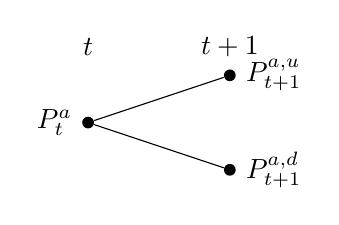
\begin{tikzpicture}[scale=1.2]
            \node (t_label) at (0,0.8) {$t$};
            \node (t1_label) at (1.5,0.8) {$t+1$};
            
            \node (t) at (0,0) [circle, fill, inner sep=1.5pt, label=left:{$P_t^a$}] {};
            \node (u) at (1.5,0.5) [circle, fill, inner sep=1.5pt, label=right:{$P_{t+1}^{a,u}$}] {};
            \node (d) at (1.5,-0.5) [circle, fill, inner sep=1.5pt, label=right:{$P_{t+1}^{a,d}$}] {};
            
            \draw (t) -- (u);
            \draw (t) -- (d);
        \end{tikzpicture}
    \end{center}

    $\to$ The result extends to any American contingent claim!
\end{remark}

\section{Continuous Time}

\begin{remark}
    \vocab{Infinite Horizon Put} (Peskir \& Shiryaev, Ch 2/11, Bjork, Ch 21)

    Generalising the results in discrete time, the arbitrage-free price of an American put is
    \[ V_s = \sup_{\tau} \EE_s \left[ e^{-r\tau} (K - S_\tau)^+ \right] = V_*(s) \]
    where $g(s) = (K-s)^+$ is the payoff function, and we consider a \vocab{Geometric Brownian Motion} (GBM) for the stock price:
    \[ dS_t = r S_t dt + \sigma S_t dW_t, \quad S_0 > 0 \text{ under } \PP^* \]
    where $r > 0$, $(W_t)_{t \geq 0}$ is a standard BM with infinitesimal generator
    \[ \mc{L}_S = r s \frac{\partial}{\partial s} + \frac{\sigma^2}{2} s^2 \frac{\partial^2}{\partial s^2} \]
    The unique solution is $S_t = S_0 e^{(r - \frac{\sigma^2}{2})t + \sigma W_t}$.

    Recall that the optimal stopping problem above is connected to the solution of a \vocab{variational inequality} and to a \vocab{free-boundary problem}:
    \[ \max \{ \mc{L}_S V(s) - r V(s), g(s) - V(s) \} = 0, \quad s \in \RR^+ \]
    Notice that the closer $S_t$ gets to zero, the greater the current exercise value and the less likely the gain function is to increase upon continuation. It is natural thus to guess that the \vocab{continuation region} $\mc{C} = (b, +\infty)$, $b \in (0, K)$, and thus if $S < b$ it will be optimal to exercise the option, i.e. the stopping time $\tau_b = \inf \{ t \geq 0 : X_t \leq b \}$ is optimal.
\end{remark}

\begin{remark}
    Thus, the free-boundary problem reads:
    \begin{enumerate}[label=(\roman*)]
        \item $\mc{L}_S V = r V$ for $s > b$ (PDE in the continuation region)
        \item $V(s) = (K-s)^+$ for $s = b$ (exercise value at a stopping time, continuity)
        \item $V(s) > (K-s)^+$ for $s > b$ (continuation)
        \item $V(s) = (K-s)^+$ for $0 < s < b$ (exercise)
        \item $V'(s) = -1$ for $s = b$ (\vocab{smooth-fit condition}) $\implies V$ is $C^1$ at $b$.
    \end{enumerate}

    Let's solve it. This will be our solution guess, which we will then verify.
    \begin{center}
        \begin{tikzpicture}
            \draw[->] (0,0) -- (4,0) node[below] {$t$};
            \draw[->] (0,0) -- (0,3) node[left] {$S_t$};
            \draw (0,1) -- (4,1) node[right] {$b$};
            \draw (0,2) -- (4,2) node[right] {$K$};
            \draw[thick] plot [smooth, tension=1] coordinates {(0,2.5) (1,2.2) (2,1.5) (3,1) (3.5,0.8)};
            \draw[dashed] (3,1) -- (3,0) node[below] {$\tau^*$};
        \end{tikzpicture}
    \end{center}
\end{remark}

\begin{remark}
    (i) reads
    \[ r s V' + \frac{\sigma^2}{2} s^2 V'' - r V = 0 \tag{*} \]
    We guess a solution of the form $V(s) = s^p$. Since $V' = p s^{p-1}$ and $V'' = p(p-1) s^{p-2}$, we substitute in (*) and obtain
    \[ r s p s^{p-1} + \frac{\sigma^2}{2} s^2 p(p-1) s^{p-2} - r s^p = 0 \]
    \[ \implies \frac{\sigma^2}{2} p^2 + p \left( r - \frac{\sigma^2}{2} \right) - r = 0 \]
    \[ p_{1,2} = \frac{-(r - \frac{\sigma^2}{2}) \pm \sqrt{(r - \frac{\sigma^2}{2})^2 + 2 \sigma^2 r}}{\sigma^2} = \frac{-(r - \frac{\sigma^2}{2}) \pm \sqrt{(r + \frac{\sigma^2}{2})^2}}{\sigma^2} \]
    where we used $(r - \frac{\sigma^2}{2})^2 + 2 \sigma^2 r = r^2 - r \sigma^2 + \frac{\sigma^4}{4} + 2 \sigma^2 r = r^2 + r \sigma^2 + \frac{\sigma^4}{4} = (r + \frac{\sigma^2}{2})^2$.
    The roots are:
    \[ p_1 = 1, \quad p_2 = -\frac{2r}{\sigma^2} \]
    The general solution of (*) then reads $V(s)=C_{1}s+C_{2}s^{-\frac{2r}{\sigma^2}}$.
\end{remark}

\begin{remark}
    Now, $\PP_s(S_t = b) = 0$ for all $s, t$ and we have that
    \[ e^{-rt}(K - S_t)^+ \leq e^{-rt} V(S_t) \leq V(s) + M_t, \quad \forall s \]
    where the first inequality follows from properties (i), (iii), and (iv) established previously, and the second follows from $(*)$. Here $(M_t)_{t \geq 0}$ is a continuous local martingale defined as
    \[ M_t = \int_0^t e^{-rs} \sigma S_s V'(S_s) dB_s. \]

    \begin{homework}
        Verify that $(M_t)_{t \geq 0}$ is indeed a martingale.
    \end{homework}

    Let $(\tau_n)_{n \geq 1}$ be a sequence of bounded stopping times for $M$. Then for any stopping time $\tau$ of $S$ we have that
    \[ e^{-r(\tau \wedge \tau_n)} (K - S_{\tau \wedge \tau_n})^+ \leq V(s) + M_{\tau \wedge \tau_n}, \quad n \geq 1. \]
    Taking $\PP_s$-expectation and noting that $\EE_s [M_{\tau \wedge \tau_n}] = 0$ by the \vocab{optional sampling theorem}, letting $n \to +\infty$, we have by \vocab{Fatou's lemma}:
    \[ \EE_s \paren{e^{-r\tau}(K - S_\tau)^+} \leq V(s). \]
    Taking the supremum over all stopping times $\tau$, we obtain
    \[ \sup_\tau \EE_s \paren{e^{-r\tau}(K - S_\tau)^+} = V_*(s) \leq V(s), \quad \forall s. \]
\end{remark}

\begin{remark}
    2) To prove $\geq$, taking $(*)$ and (i) and using again the optional sampling theorem we have that, $\forall \tau$ and for $\tau_b$
    \[ \EE_s \paren{ e^{-r(\tau_b \wedge \tau_n)} V(S_{\tau_b \wedge \tau_n}) } = V(s) \quad \forall n \geq 1 \]
    Letting $n \to \infty$, since $e^{-r\tau_b} V(S_{\tau_b}) = e^{-r\tau_b} (K - S_{\tau_b})^+$, by dominated convergence we have
    \[ \EE_s \paren{ e^{-r\tau_b} (K - S_{\tau_b})^+ } = V(s). \]
    $\implies \tau_b$ is optimal and $V_*(s) = V(s) \quad \forall s > 0$. $\square$
\end{remark}

\section{Finite Horizon}

\begin{remark}
    \vocab{FINITE HORIZON}
    
    The finite horizon case is not so analytically tractable as the infinite horizon one.
    
    The problem becomes
    \[ V(t,s) := \sup_{0 \leq \tau \leq T-t} \EE_{t,s} \left[ e^{-r\tau} (K - S_{t+\tau})^+ \right] \]
    where $\tau$ is a stopping time.
    \[ dS_{t+u} = r S_{t+u} du + \sigma S_{t+u} dB_u, \quad S_t = s > 0 \]
    Here again (see 1st part of the course) we have a variational inequality:
    \[ \max \left\{ g(s) - V(t,s), \frac{\partial V(t,s)}{\partial t} + \mc{L}_X V(t,s) - r V(t,s) \right\} = 0 \]
    for $(t,s) \in [0,T) \times \RR^d$, with $V(T,s) = g(s)$.
    
    The problem is, in this case, bi-dimensional.
\end{remark}

\begin{remark}
    In this case, the \vocab{continuation region} is
    \[ \mc{C} = \{ (t,s) \in [0,T) \times (0, \infty) : V(t,s) > g(s) \} \]
    while the \vocab{stopping set} is
    \[ \bar{D} = \{ (t,s) \in [0,T] \times (0, \infty) : V(t,s) = g(s) \} \]
    and $\tau_D^* = \inf \{ 0 \leq u \leq T-t : X_{t+u} \in \bar{D} \}$ is the optimal stopping time.
    
    It is possible to prove that:
    \begin{enumerate}[label=\alph*)]
        \item $\exists b : [0,T] \to \RR$ s.t.
        \[ \mc{C} = \{ (t,s) \in [0,T] \times (0, \infty) : s > b(t) \}, \]
        $\bar{D}$ is the closure of $D = \{ (t,s) \in [0,T] \times (0, \infty) : s \leq b(t) \}$.
        \item $V(t,s)$ is decreasing on $[0,T]$ for each $s \in (0, \infty)$ and $t \to b(t)$ is increasing on $[0,T]$.
        \item $(t,s) \to V(t,s)$ is continuous.
        \item $s \to V(t,s)$ is $C^1$ at $b(t)$.
        \item $b$ is continuous on $[0,T]$ and $b(T) = K$.
    \end{enumerate}
\end{remark}

\begin{remark}
    \begin{center}
        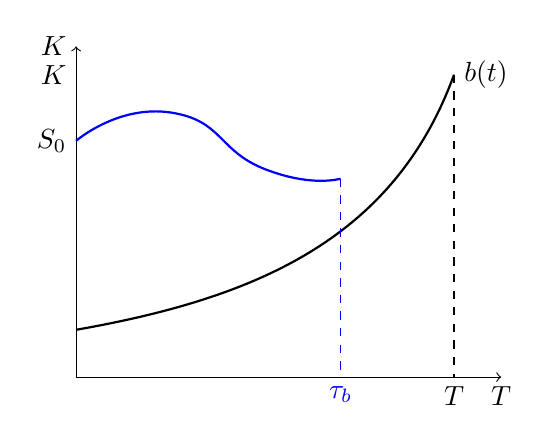
\begin{tikzpicture}[scale=1.2]
            \draw[->] (0,0) -- (4.5,0) node[below] {$T$};
            \draw[->] (0,0) -- (0,3.5) node[left] {$K$};
            \node at (0,3.2) [left] {$K$};
            \node at (0,2.5) [left] {$S_0$};
            \draw[thick] (0,0.5) to[out=10, in=-110] (4,3.2) node[right] {$b(t)$};
            \draw[dashed] (4,3.2) -- (4,0) node[below] {$T$};
            \draw[blue, thick] plot [smooth, tension=1] coordinates {(0,2.5) (1,2.8) (2,2.2) (2.8,2.1)};
            \draw[blue, dashed] (2.8,2.1) -- (2.8,0) node[below] {$\tau_b$};
        \end{tikzpicture}
    \end{center}
    
    Hence, it follows that we have the following free-boundary problem for the unknown value function $V$ and boundary $b$:
    \begin{align*}
        V_t + \mc{L}_S V &= r V && \text{in } \mc{C} \\
        V(t,s) &= (K-s)^+ && s = b(t) \\
        V_s(t,s) &= -1 && s = b(t) \quad \text{$\to$ smooth fit, guarantees $V$ is $C^{1,2}$ in $\mc{C}$, $C^1$ in $D$} \\
        V(t,s) &> (K-s)^+ && \text{in } \mc{C} \\
        V(t,s) &= (K-s)^+ && \text{in } D
    \end{align*}
    \begin{itemize}
        \item $\tau^* = \inf \{ t \geq 0 : S_t = b(t) \}$ is the optimal stopping time.
    \end{itemize}
\end{remark}

\begin{remark}
    No analytical formula is available. Alternatives:
    \begin{enumerate}
        \item Solve the free-boundary problem numerically.
        \item Solve the variational inequalities.
        \item Approximate via a binomial model and compute the binomial price.
    \end{enumerate}
\end{remark}